\documentclass[a4paper,12pt,french] {article}

\usepackage{../../../../Style}

\renewcommand\tabularxcolumn[1]{m{#1}}

\geometry{bottom=23mm}
\pagestyle{fancy}
\setlength{\headheight}{10mm}
\fancyhead[L]{2021-2022}
\fancyhead[C]{\textbf{Devoir supplémentaire: Fonctions - Généralités}}
\fancyhead[R]{\premiere ST2S 2}
\fancyfoot[C]{Page \thepage}

\usepackage{icomma}

\renewcommand{\baselinestretch}{1.25}

\setlist[itemize]{align=parleft,left=5pt..15pt}
\setlist[enumerate]{align=parleft,left=5pt..20pt}

\begin{document}

\rem{L'usage de la calculatrice est autorisé. La propreté et l'orthographe seront prises en compte. Tout le devoir peut être fait sur le sujet.}

Nom: \hfill Prénom: \hfill \

\begin{exercice} \

\compo[0.4]
{
\begin{center}
\vspace{3mm}
Questions 2 et 3
\begin{tikzpicture}
\begin{axis}[
styleglobal,
width=\linewidth,
xmin=-2.5, xmax= 6.5,
ymin=-1.5, ymax=4.5,
xtick distance=1,
ytick distance=1,
]
\addplot[samples=101,smooth,line width=1.3pt,domain=(0:4),mark=none] plot coordinates {(-2,-1) (-1,1) (0.2,2.7) (1,1) (2,-1) (3,0) (4.5,3.5) (6,2.7)} node[pos=0.9,above right] {$\mathscr C_f$}  \pointsextremites;
\end{axis}
\end{tikzpicture}

\vspace{3mm}
Questions 4 et 5
\begin{tikzpicture}
\begin{axis}[
styleglobal,
width=\linewidth,
xmin=-2.5, xmax= 6.5,
ymin=-1.5, ymax=4.5,
xtick distance=1,
ytick distance=1,
]
\addplot[samples=101,smooth,line width=1.3pt,domain=(0:4),mark=none] plot coordinates {(-2,-1) (-1,1) (0.2,2.7) (1,1) (2,-1) (3,0) (4.5,3.5) (6,2.7)} node[pos=0.9,above right] {$\mathscr C_f$}  \pointsextremites;
\end{axis}
\end{tikzpicture}
\end{center}
}
{
On a représenté une fonction $f$ sur le repère ci-contre. Des constructions sont demandées pour les questions indiquées.
\begin{enumerate}
\item L'ensemble de définition de $f$ est $\dotfill$
\item L'image de 2 est \dotfill
\item L'image de -1 est \dotfill
\item $1$ a pour antécédent(s) \dotfill
\item $2,5$ possède \makebox[3cm]{\dotfill} antécédent(s).
\item Dresser un tableau de signes de la fonction $f$.
\item Dresser un tableau de variations de la fonction $f$.
\end{enumerate}
\begin{center}
\begin{tabularx}{0.9\linewidth}{|c|X|} \hline
\rule{0pt}{25pt} & \\ \hline
\phantom{f(x)} & \rule{0pt}{25pt}\\ \hline
\end{tabularx}

\vspace{3mm}

\begin{tabularx}{0.9\linewidth}{|c|X|} \hline
\rule{0pt}{25pt} & \\ \hline
\phantom{f(x)} & \rule{0pt}{75pt}\\ \hline
\end{tabularx}
\end{center}
}
\end{exercice}

\begin{exercice}
Soit $f$ une fonction définie sur un ensemble $D$. On note $\mathscr C_f$ sa courbe représentative dans un repère. Compléter le tableau suivant:

\vspace{2mm}

\setlength{\extrarowheight}{-5pt}
\renewcommand{\arraystretch}{4}
\setstretch{1}{
\noindent\begin{tabularx}{\linewidth}{|c|*{3}{Y|}} \hline
\ Egalité \ & Image & Equation & Antécédent \\ \hline $f(2)=3$ & & & \\ \hline & $1$ a pour image $0$ par $f$ & & \\ \hline & & $4$ est une solution de l'équation $f(x)=5$ & \\ \hline & & & 3 est un antécédent de $-4$ par $f$\\ \hline
\end{tabularx}}

\end{exercice}

\begin{exercice}
Soit $f:[0;5] \rightarrow \R$ la fonction qui a $x$ associe $\frac {8x-2}{x+1}$.

\compo[0.7]
{
\begin{enumerate}
\item Compléter le tableau de valeurs suivant, en arrondissant au dixième près:

\begin{center}
\begin{tabularx}{0.9\linewidth}{|c|*{6}{Y|}} \hline
$x$ & $0$ & $1$ & $2$ & $3$ & $4$ & $5$ \\ \hline
$f(x)$ & & & & & & \rule{0pt}{8mm} \\ \hline
\end{tabularx}
\end{center}
\item Tracer sur le repère ci-contre la représentation graphique de $f$.
\item Le point $(2,5 \, ; \, 5,5)$ appartient-il à la courbe de $f$? Justifier par un calcul.

\points 3

\item Calculer le taux de variations de $f$ entre $2$ et $4$, puis entre $0$ et $5$.
\end{enumerate}
}
{
\begin{tikzpicture}
\begin{axis}[
styleglobal,
width=\linewidth,
xmin=-0.5, xmax= 5.5,
ymin=-2.5, ymax=7,
xtick distance=1,
ytick distance=1,
]

\end{axis}
\end{tikzpicture}
}
\vspace{15pt}
\points 3
\end{exercice}

\begin{exercice} \

\compo[0.6]
{
On a représenté deux fonctions $f$ et $g$ sur le repère ci-contre. Résoudre graphiquement les (in)équations suivantes:
\begin{enumerate}
\item $f(x) \geq 0$: \dotfill
\item $f(x)=g(x)$: \dotfill
\item $f(x) < g(x)$: \dotfill
\end{enumerate}
}
{
\begin{center}
\begin{tikzpicture}
\begin{axis}[
styleglobal,
width=\linewidth,
xmin=-4, xmax= 4,
ymin=-2, ymax=3,
xtick distance=1,
ytick distance=1,
]
\addplot[samples=101,smooth,line width=1.3pt,domain=(0:4),mark=none] plot coordinates {(-3,2) (-2.5,1) (-1,0) (1,2.5) (3,1)} node[pos=0.9,above right] {$\mathscr C_f$}  \pointsextremites;
\addplot[color=blue,densely dashed,samples=101,smooth,line width=1.3pt,domain=(-3:3),mark=none] plot {(2-0.25*x^2)*(1.2-e^(0.8*x-1.5))-0.5} node[pos=0.85,below] {$\mathscr C_g$}  \pointsextremites;
\end{axis}
\end{tikzpicture}
\end{center}
}

\end{exercice}

\begin{exercice} \
Pour chacun de ces quatre récipients, associer la courbe donnant le volume $V$ de liquide en fonction de sa hauteur $h$ dans le récipient.

\compo[0.25]
{
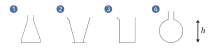
\includegraphics[width=\linewidth]{ExoDSAssociation1.png}
}
{
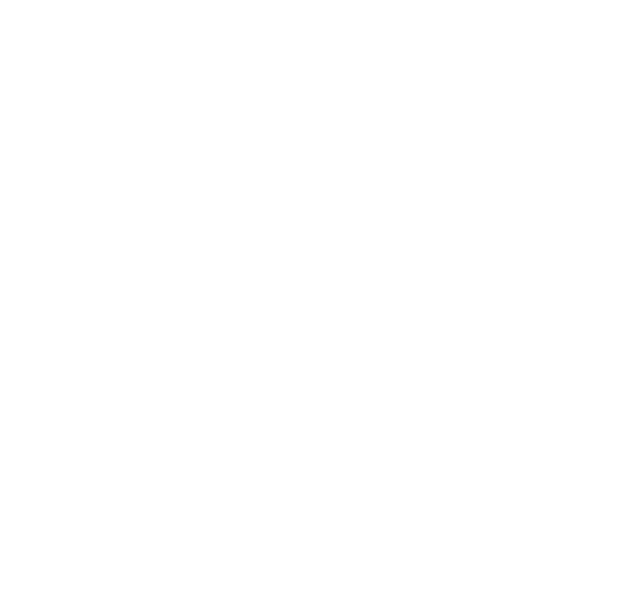
\includegraphics[width=\linewidth]{ExoDSAssociation2.png}

\ \hfill \ldots \hfill \hfill \ldots \hfill \hfill \ldots \hfill \hfill \ldots \hfill \
}
\end{exercice}



\begin{comment}

\begin{exercice}
Problème avec lecture graphique image, antécédent, résolution équation, tableaux signe variation, tx variation

Par exemple production de deux entreprises avec deux fonctions, à mettre sur le même graphe?

Bénéfices de deux entreprises pendant 

\begin{center}
\begin{tikzpicture}[scale=0.8]
\begin{axis}[
styleglobal,
width=\linewidth,
xmin=0, xmax= 30,
ymin=-1, ymax=4.5,
xlabel={Temps (en jours)},
ylabel={Population},
minor x tick num=1,
minor y tick num=1,
ytick distance=2,
xtick distance=1,
yscale=0.5
]
\addplot[samples=101,smooth,ultra thick,mark=none] plot coordinates {(0,0) (0.5,4) (1,0) (2,-1) (4,0) (5,2)};

\end{axis}
\end{tikzpicture}
\end{center}

\end{exercice}

\begin{exercice}
Tableau de variations et de signes
\end{exercice}

\end{comment}

\end{document}